\documentclass[Main.tex]{subfiles} 
\begin{document}

\subsection{Oversigt over processer/task}
Processen p� PC'en best�r samlet set af 6 tr�de.\\
\begin{figure}[H]
\centering
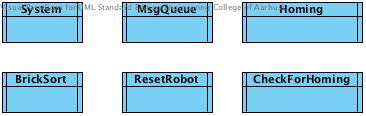
\includegraphics[scale=1]{Billeder/ProcesTaskView.jpg}
\caption{Oversigt over tr�de}
\end{figure}
\textbf{System} - Hovedtr�d som starter og initialiserer robotten. Tr�den s�rger ogs� for brugergr�nsefladen.\\ 
\textbf{MsgQueue} - Opretter en besked k� som bruges til at sende eller modtage beskeder til og fra databasen.\\
\textbf{Homing} - Tr�d som g�r at robotten kan home igennem brugergr�nsefladen.\\
\textbf{BrickSort} - Tr�d der s�rger for at sortere de forskellige klodser.\\
\textbf{ResetRobot} - Tr�d der g�r det muligt at stoppe programmet i en given sekvens igennem brugergr�nsefladen, hvorefter den returnere til startpositionen.\\
\textbf{CheckForHoming} - Tr�d der tjekker hvorn�r robotten er homet.\\
\end{document}